\chapter{Implementation}

\section{Used Techrnologies}
\subsection{Standard Widget Toolkit (SWT)}

SWT\footnote{http://www.eclipse.org/swt/} is an open source library for creating graphical user interfaces. The project was initiated 2001 by IBM under within the scope of the Eclipse framework\footnote{http://www.eclipse.org}. In contrast to the standard Java toolkits like the Abstract Widget Toolkit (AWT) and Swing took the SWT designer an approach which is closer to the native operating system widgets. This results in a better performance and a native look of the widgets.

\subsection{JOGL}

Java OpenGL library\footnote{https://jogl.dev.java.net/}
[Compare to Java3D]

%\subsection{OpenGL integration in Java}
\subsection{JGraph}

\section{Data loading}

KEGG provides the data the XML (Extensible Markup Language) file format which made the job easy to parse the data in Java. We had to face the choice between between several ways of parsing offered by the Java Standard API. 
Most relavant methods are\cite{Niemeyer2002}:
\begin{itemize}
 \item \textbf{Simple API for XML (SAX):}\\
  TODO: Describe SAX here
 \item \textbf{Document Object Model (DOM):}\\
  TODO: Describe DOM here
\end{itemize}

KEGG pathway are defined in the KEGG Markup Language (KGML)\footnote{http://www.genome.jp/kegg/docs/xml/}.
KGML mixes information about the map structure and the visual representation (like colors, shapes, etc.).
Here is a snip of the example pathways Methionine Metabolism in KGML stored in a XML file:

\begin{verbatim}
<pathway name="path:map00271" org="map" number="00271" 
title="Methionine metabolism" 
image="http://www.genome.jp/kegg/pathway/map/map00271.gif" 
link="http://www.genome.jp/dbget-bin/show_pathway?map00271">

  <entry id="1" name="ec:2.6.1.-" type="enzyme" reaction="rn:R07396"
  link="http://www.genome.jp/dbget-bin/www_bget?enzyme+2.6.1.-">
    <graphics name="2.6.1.-" fgcolor="#000000" bgcolor="#FFFFFF" type="rectangle" 
    x="335" y="571" width="45" height="17"/>
  </entry>

  <entry id="2" name="cpd:C08276" type="compound" 
  link="http://www.genome.jp/dbget-bin/www_bget?compound+C08276">
    <graphics name="C08276" fgcolor="#000000" bgcolor="#FFFFFF" type="circle" 
    x="466" y="494" width="8" height="8"/>
  </entry>
  ...
  <reaction name="rn:R01402" type="irreversible">
    <substrate name="cpd:C00170"/>
    <product name="cpd:C04188"/>
  </reaction>
  ...
</pathway>
\end{verbatim}

The alternative would habe been the usage of the KEGG application programming interface (API). The in Java implemented API employs the Simple Object Access Protocol (SOAP) for the transfer of XML information over HTTP. Due to the fact that real-time behaviour is in the main focus of the framework the SOAP alternative was too slow.

Problem of double data keeping. 

\section{Visualization techniques}

In the upcoming section used visualization methods are described and their realization is going to be discussed. Basically the section is divided in 2D pathway implementation and the 3D OpenGL pathways.

\subsection{2D pathway implementation}

\begin{figure}[ht]
  \centering
    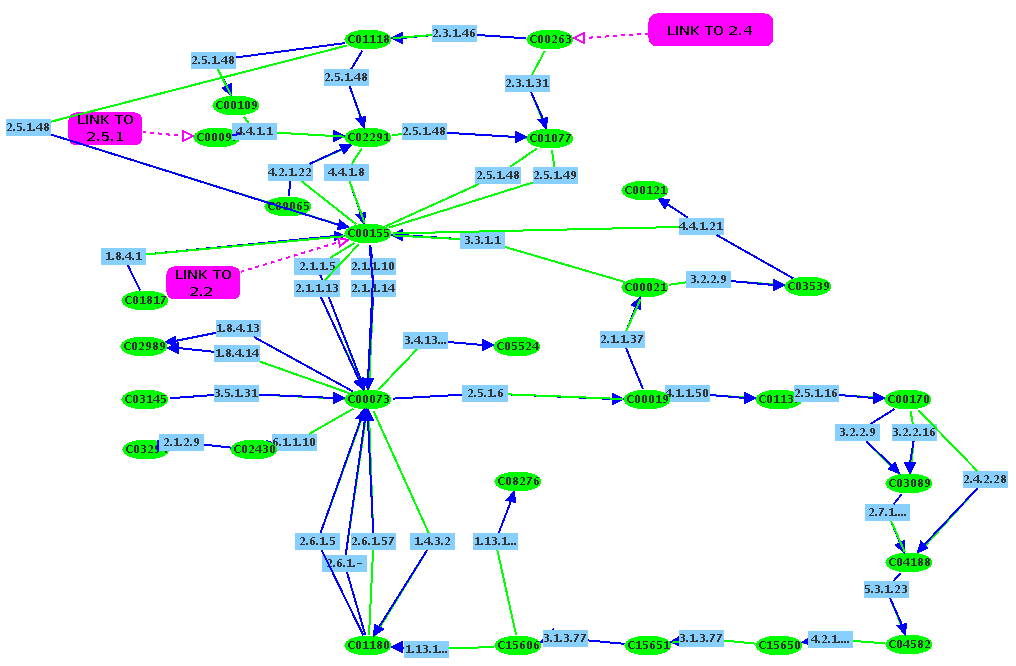
\includegraphics[width=0.7\linewidth]{gfx/sample_pathway_jgraph}
  \caption{Sample pathway without any layouting modification.}
  \label{fig:sample_pathway_jgraph}
\end{figure}

\begin{figure}[ht]
  \centering
    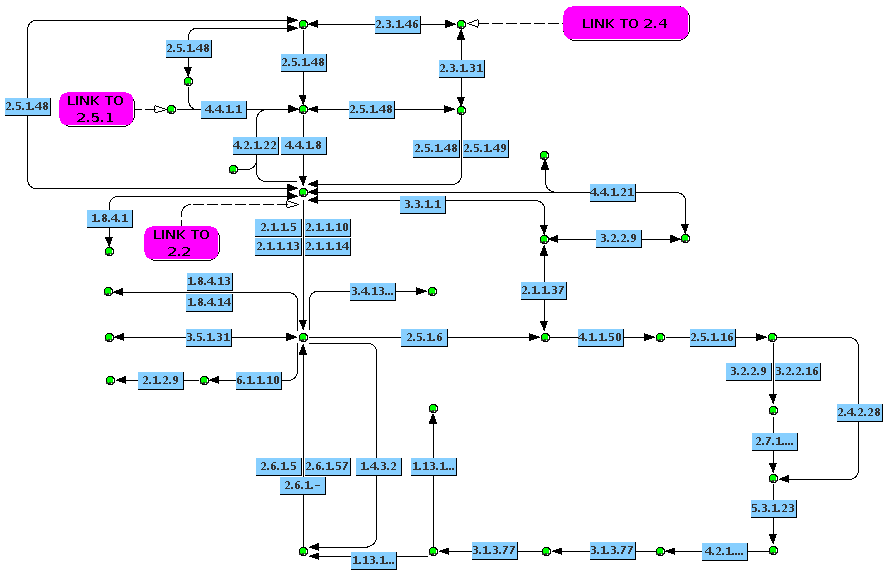
\includegraphics[width=0.7\linewidth]{gfx/sample_pathway_jgraph_background}
  \caption{Sample pathway with background texture overlay (FIX screeny: labels are missing!).}
  \label{fig:sample_pathway_jgraph_background}
\end{figure}

The context information where in the hierarchical KEGG levels the presented piece of information is located would lead to a better orientation inside the metabolic network \cite{Jourdan2003}. Therefore this feature can be seen as a valuable extension for the future. 

\subsubsection{Pathway switching}
\label{ssec:pathway_switching}

Pathways are linked to related pathways. In the KEGG drawing style linked maps are represented by roundrectangular nodes inside pathway graphs. Therefore it is important to support fast switching between them. We implementing the switching action by replacing the currently shown graph which is triggered by a mouse event. This mechanism enables the user to freely navigate inside the metabolic network.

\subsubsection{Hierarchical pathways}

KEGG added two abstraction levels above the metabolic pathways. The pathways are categorized in 10 groups which represent the highest layer. The middle level...
\stdref{gfx:KEGG_abstraction_chain} shows the three KEGG abstraction levels. 
In the webbased KEGG version each abstract level has an imagemap in the back. In the imagemap rectangular portions are defined and provided with a hyperlink to the next layer below. We use the same mechanism for linking pathways between abstraction levels. In contrast to KEGG we store the imagemap information in XML which is parsed at bootstrapping. During runtime when a mouse event is triggered on the 2D pathway the clicked position is checked if it is contained in a predefined area. If a positive match is found the link for this area is returned and the requested next layer map can be loaded.

\begin{figure}[ht]
\centering
\scalebox{0.35}{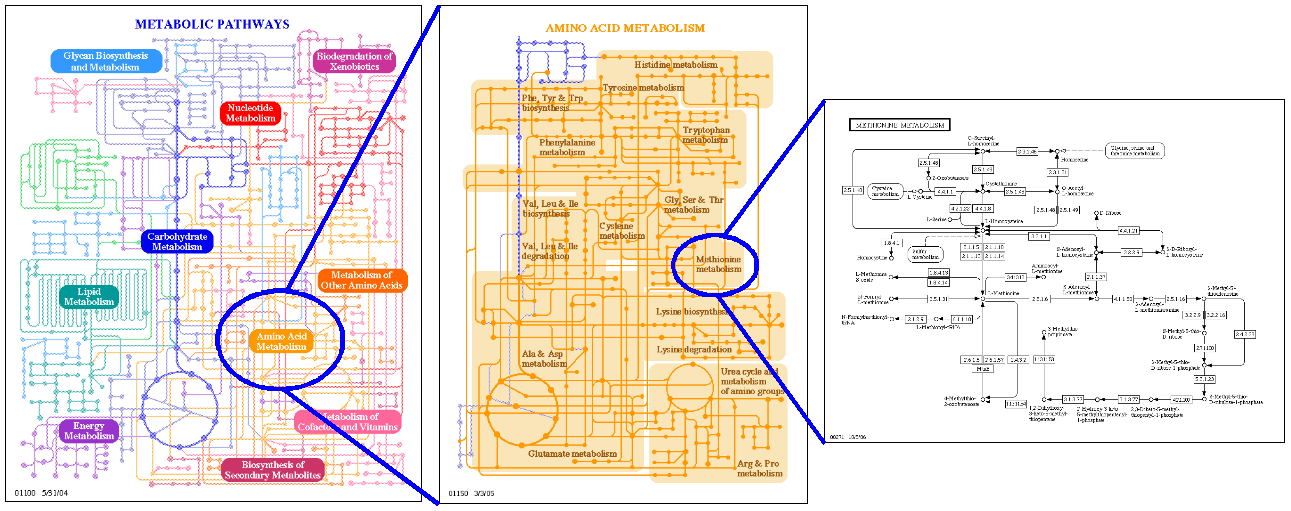
\includegraphics{gfx/KEGG_abstraction_chain}} 
\caption[KEGG abstraction chain]{\textit{KEGG abstraction chain}} 
\label{gfx:KEGG_abstraction_chain}
\end{figure}

\subsubsection{Neighborhood visualization}

In graphs where the layout aims on the positioning of nodes and edges to circumvent intersections neighborhood visualization occupies an important role. The geographic position of nodes is independent from their relational distance. Hence far away positioned nodes can be directly related to a node in focus whereas near nodes are e.g. several indirections away. 

We implemented the neighborhood visualization using a modified Breadth-first-search (BFS) approach\cite{Cormen2001}. The BFS algorithm visits all direct neighbors. After that procedure for each neighbor the same strategy is applied. If an already visited node is inspected it will be ignored. This assures that only the shortest path to a node is considered (for unweighted graphs). The algorithm is applicable on undirected and directed graphs.
The alogrithm can be executed for arbitrary depth. Neighborhood coloring up to the depth of 3 seems to be the limit. The application of farer away neighborhood distances entails confusion at user's side because of the cyclic charakter of the graphs. 
The neighborhood algorithm for a distance of 3 is applied on the sample Methionine Metabolism pathway in \stdref{gfx:neighborhood_visualization_distance_3}. The selected node is colored red. The neighboring nodes are shaded from orange (distance 1) to light yellow (distance 3).

Elements visited by the neighborhood algorithm can form a so called selection. Afterwards the selection can be propagated to other dependent views by using the update-mechanism (FULLREF).

\begin{figure}[ht]
\centering
\scalebox{0.5}{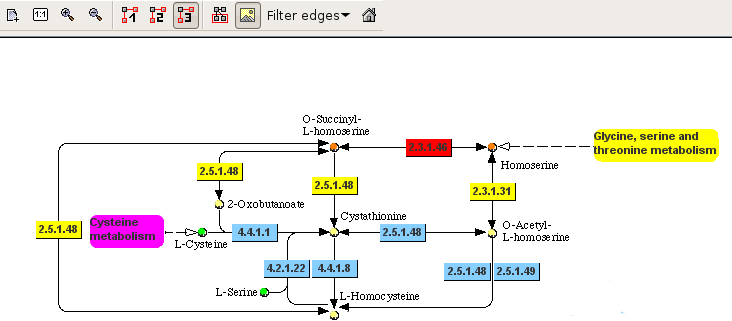
\includegraphics{gfx/neighborhood_visualization_distance_3}} 
\caption[Distance 3 neighborhood visualization]{\textit{Distance 3 neighborhood visualization}} 
\label{gfx:neighborhood_visualization_distance_3}
\end{figure}

\begin{figure}[ht]
  \centering
    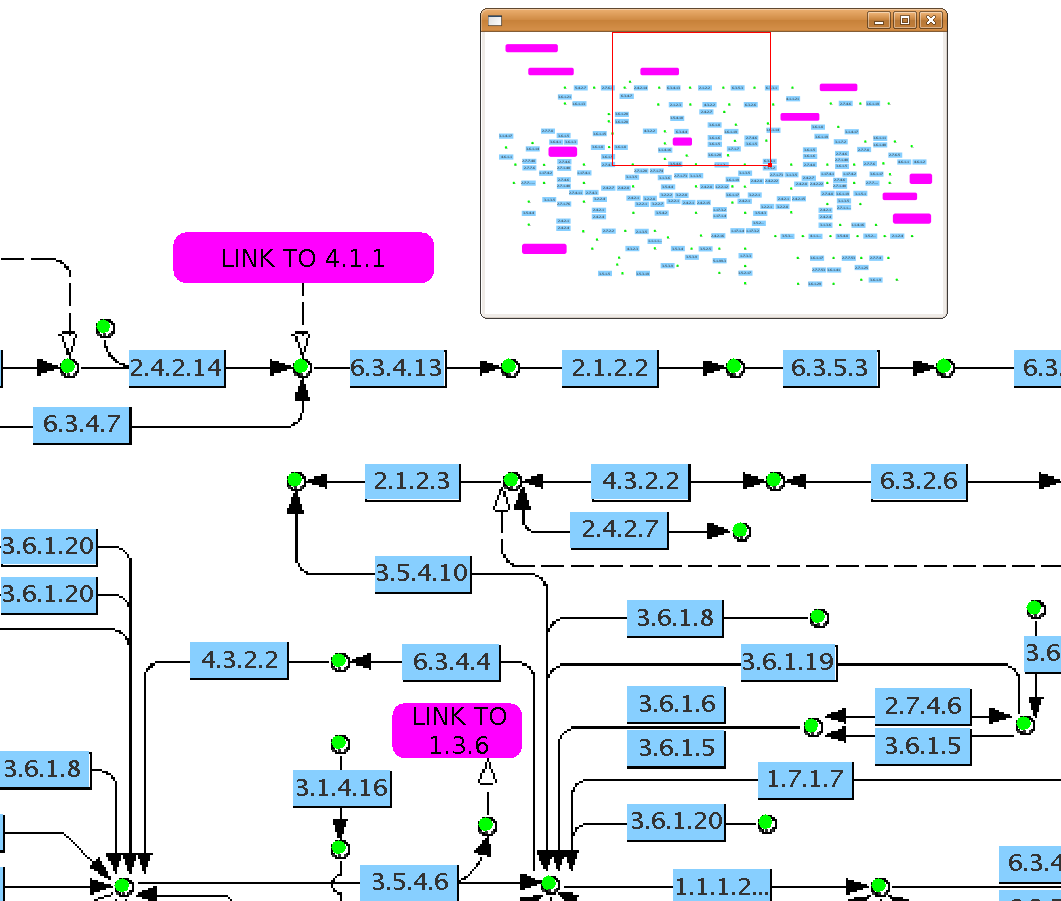
\includegraphics[width=0.5\linewidth]{gfx/overview_method}
  \caption{Portion of a sample pathway that can be interactively selected in the overview map.}
  \label{fig:overview_method}
\end{figure}

\subsection{3D OpenGL pathways}

\begin{figure}
  \centering
    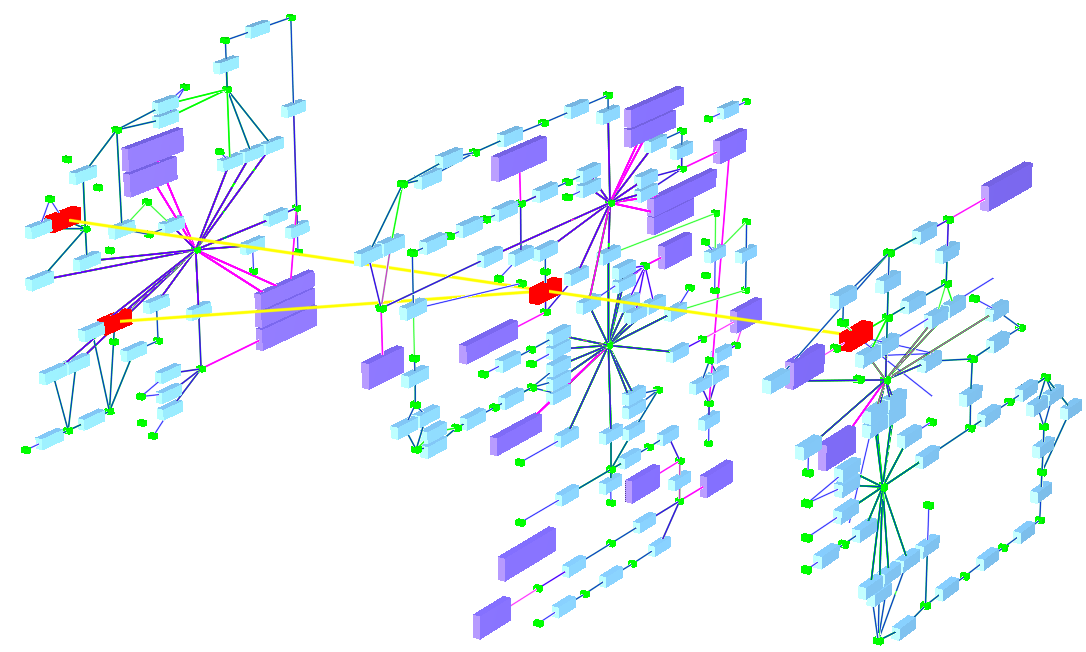
\includegraphics[width=0.7\linewidth]{gfx/opengl_layered_pathway_without_texture}
  \caption{2.5-D OpenGL layered pathway with a user selection}
  \label{fig:opengl_layered_pathway_without_texture}
\end{figure}

\subsubsection{Hierarchical display lists}

The purpose of display lists is to group primitive objects for later usage. The group of objects is transfered to graphic card memory in the initialization face. Thus the object can be reused wihtout the expensive transfere operation.Especially for compound objects that occur multiple times in the scene the application of display lists can significantly boost the performance. In the case of pathways the scene is built up of hundreds of enzymes and chemical compounds which are simply depicted as differently coloured cubes. A complete pahtway can be created out of these primitive objects which are again stored in a display list. Using this approach results in hierachical display lists wherd display lists are nested in higher level display lists. This empoweres us to position a specific pathway more than once in the scene without sending all primitves through the graphics pipeline. 
 
\subsubsection{Pathway texture overlay}

\begin{figure}[ht]
  \centering
    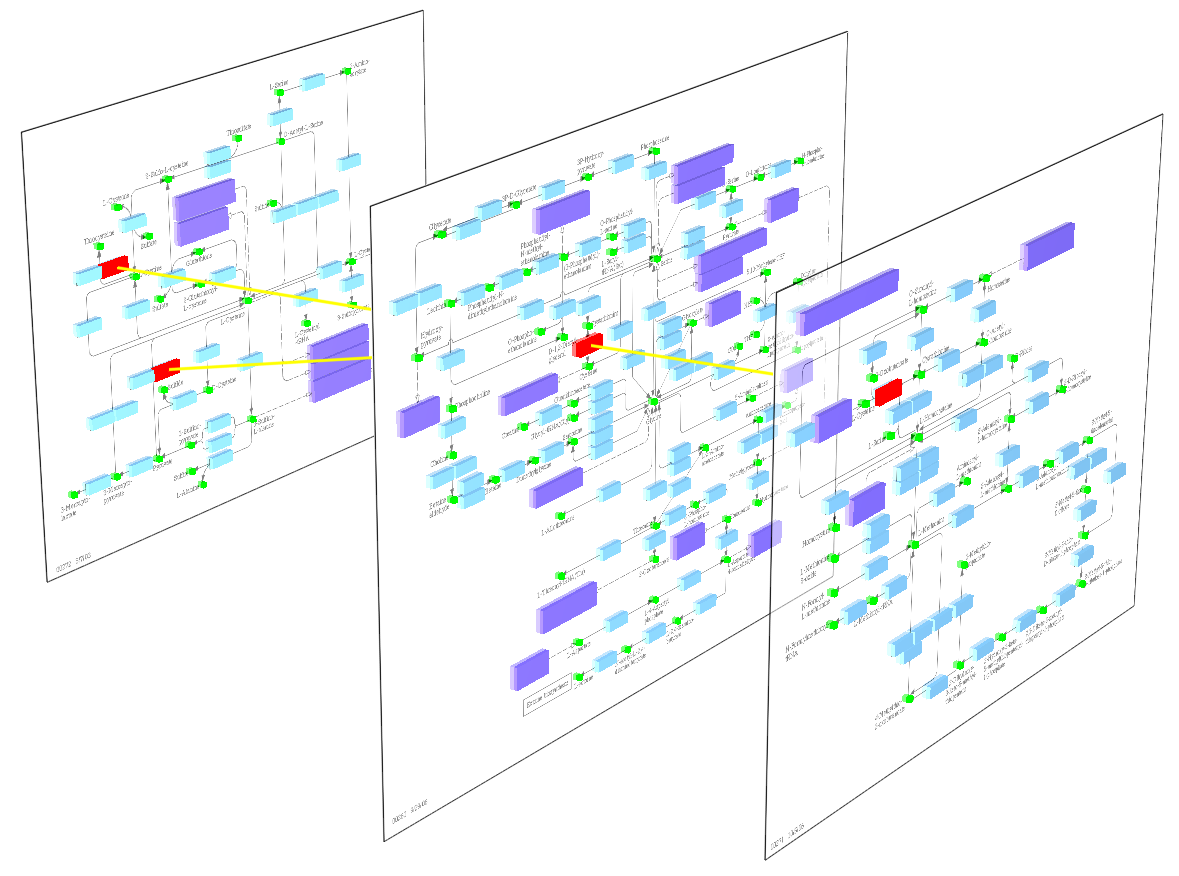
\includegraphics[width=0.8\linewidth]{gfx/opengl_layered_pathway}
  \caption{2.5-D OpenGL layered pathway with a blended texture overlay. The node in the middle layer is picked by a mouse-click event. Identical nodes in dependent graphs are interactively highlighted and connected to the selected one.}
  \label{fig:opengl_layered_pathway}
\end{figure}

\subsubsection{Showcase layouts}

Caching the model-view matrix per pathway allows a free aranchement of the planar graphs in 3D space.
This approaches enabled us to implemented two simple exemplary setups.

\minisec{Layered pathway setup}

[Insert screenshot of a layered view]

\minisec{Planar pathway setup}

One graph in the center of user interaction. Metapher of a gallery.

[Insert screenshot]


\subsubsection{Pathway switching}

Navigating through the metabolic network by exchanging pathways is basically similar to the 2D version (see \fullref{ssec:pathway_switching}). The difference lies in the implementation. In a view containing a 2D pathway a switching operation clears the old pathway and paints the new one onto the canvas. As only one pathway can be shown at the same time this strategy is implemented straight forward. In contrast in 3D space an arbitrary amount of pathways is placed in the scene. The planar graphs might differ in rotation, orientation, perspective and/or scaling factor. Figure (TODO) shows an artificial scene. Important is the fact that the visualization features (e.g. element picking, highlighting, etc.) are fully working without any modification in the code. We were able to achieve this solution by storing the model-view (??) matrix at the upper left corner of the graph plane. This approach made it easy to replace pathways without any problems.

\subsubsection{Pathway element picking}

Picking is the operation of selecting a objects in the scene. In our case we employ the picking action to select nodes inside the graphs. In OpenGL element picking can be achieved by different methods. The straight forward approach uses the OpenGL build in selection mode\cite{Shreiner2005}. The user starts the picking operation by triggering a mouse-click event. The selection mode is entered and an area around the clicked x,y screen-coordinates is defined by appliying a picking matrix on the current matrix stack. Accordingly this region is then used by the selection render mode to restrict the rendered area. In selection mode the render method returns a hit record which contains the information about the intersecting objects inside the region. The size of the region determines the sensitivity of the selection.  

In addition to the described method we used hierarchical object picking. In that case multiple names are returned for each hit. Applied to our use case the scene is made-up of several pathway graphs which represent the top-level elements in the hierarchy. In turn vertices inside the graph are on the second level. Hence the picking result gives us exact information which node in which pathway the user is interested in.

Increasing the number of visualized pathways in one scene also raises the probability of multiple objects under the curser. Therefore a picking action returns a set of hits. As each hit comes with a depth value the one which is nearest to the viewport is taken.

\subsubsection{Element highlighting \& linking}

\subsubsection{Enzyme-gene mapping}

Multi hash maps (describe)\\
Templated hash maps parametrized by data type\\
For time series experiment the index remains the same - just the pointer to the storage is replaced\\